\documentclass[tikz,border=4pt]{standalone}

\usepackage{times}
\usepackage{tikz}
\usetikzlibrary{arrows.meta,backgrounds,calc,fit,positioning}

\begin{document}
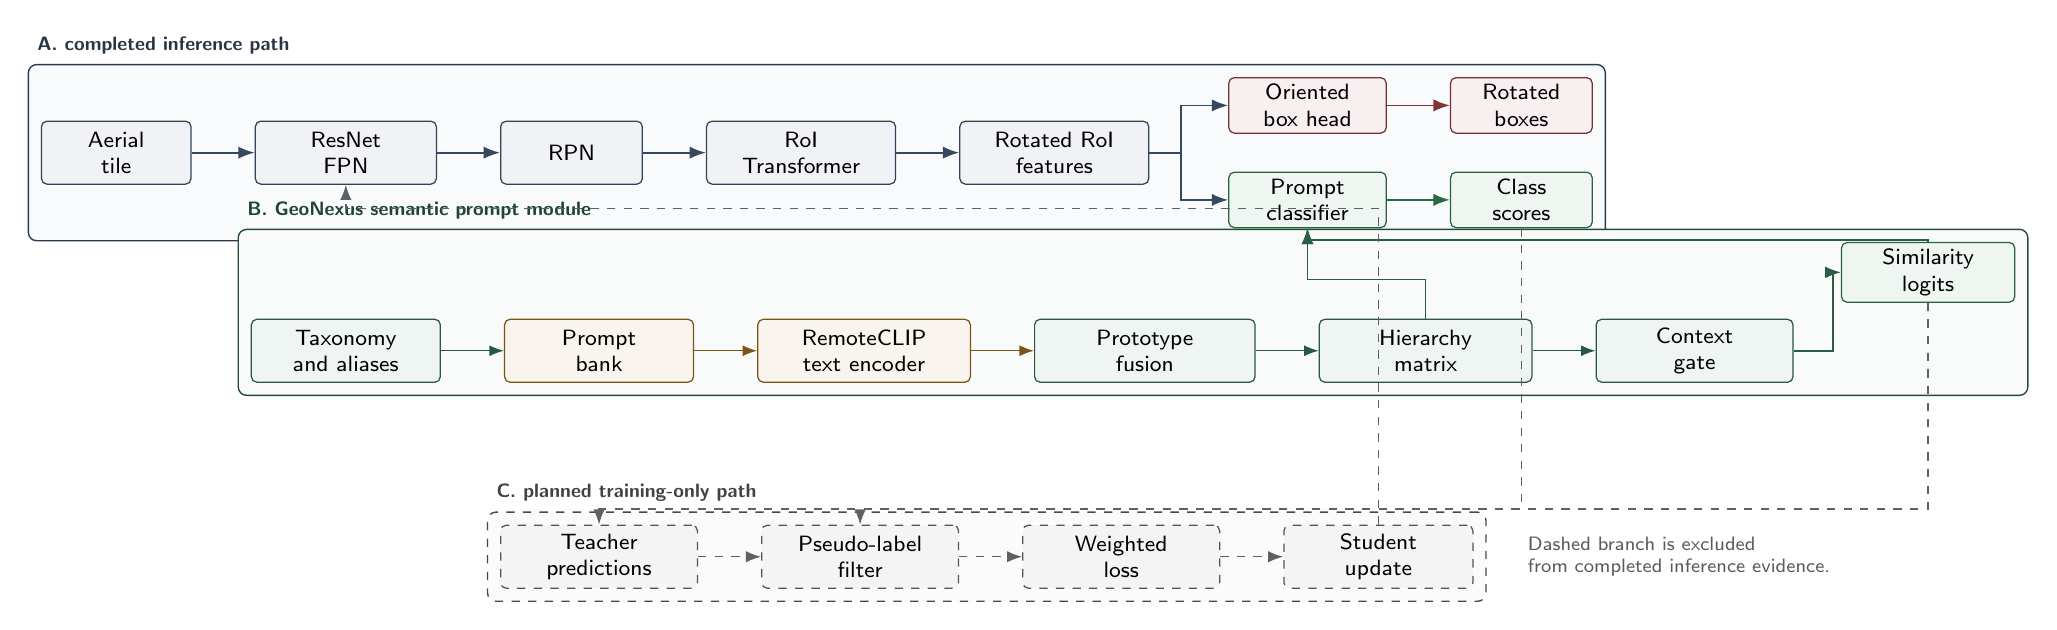
\begin{tikzpicture}[
    font=\sffamily\footnotesize,
    >=Latex,
    node distance=7mm and 8mm,
    box/.style={
        draw=#1!70!black,
        fill=#1!8,
        rounded corners=2pt,
        minimum height=8mm,
        minimum width=20mm,
        align=center,
        inner sep=3pt,
        line width=0.45pt
    },
    box/.default=bluegray,
    smallbox/.style={
        draw=#1!70!black,
        fill=#1!8,
        rounded corners=2pt,
        minimum height=7mm,
        minimum width=17mm,
        align=center,
        inner sep=2.5pt,
        line width=0.45pt
    },
    smallbox/.default=bluegray,
    group/.style={
        draw=#1!60!black,
        fill=#1!3,
        rounded corners=3pt,
        inner sep=4.5pt,
        line width=0.5pt
    },
    group/.default=bluegray,
    label/.style={font=\sffamily\scriptsize\bfseries, text=#1!55!black},
    label/.default=bluegray,
    flow/.style={->, line width=0.65pt, draw=#1!75!black},
    flow/.default=bluegray,
    softflow/.style={->, line width=0.5pt, draw=#1!70!black},
    softflow/.default=greenpath,
    planned/.style={->, dashed, line width=0.55pt, draw=plannedgray!80!black},
    join/.style={-{Latex[length=2.0mm]}, line width=0.55pt, draw=#1!75!black},
    join/.default=greenpath
]

\definecolor{bluegray}{RGB}{70,96,126}
\definecolor{greenpath}{RGB}{56,126,91}
\definecolor{amberpath}{RGB}{176,120,32}
\definecolor{plannedgray}{RGB}{116,121,127}
\definecolor{redaccent}{RGB}{166,70,70}
\definecolor{greenaccent}{RGB}{55,140,93}

% A. Completed detector inference path
\node[box=bluegray, minimum width=19mm] (tile) {Aerial\\tile};
\node[box=bluegray, right=of tile, minimum width=23mm] (backbone) {ResNet\\FPN};
\node[box=bluegray, right=of backbone, minimum width=18mm] (rpn) {RPN};
\node[box=bluegray, right=of rpn, minimum width=24mm] (roit) {RoI\\Transformer};
\node[box=bluegray, right=of roit, minimum width=24mm] (rroi) {Rotated RoI\\features};
\node[smallbox=redaccent, right=10mm of rroi, yshift=6mm, minimum width=20mm] (boxhead) {Oriented\\box head};
\node[smallbox=greenaccent, right=10mm of rroi, yshift=-6mm, minimum width=20mm] (clshead) {Prompt\\classifier};
\node[smallbox=redaccent, right=8mm of boxhead, minimum width=18mm] (boxes) {Rotated\\boxes};
\node[smallbox=greenaccent, right=8mm of clshead, minimum width=18mm] (classes) {Class\\scores};

\draw[flow=bluegray] (tile) -- (backbone);
\draw[flow=bluegray] (backbone) -- (rpn);
\draw[flow=bluegray] (rpn) -- (roit);
\draw[flow=bluegray] (roit) -- (rroi);
\draw[flow=bluegray] (rroi.east) -- ++(4mm,0) |- (boxhead.west);
\draw[flow=bluegray] (rroi.east) -- ++(4mm,0) |- (clshead.west);
\draw[flow=redaccent] (boxhead) -- (boxes);
\draw[flow=greenaccent] (clshead) -- (classes);

\begin{pgfonlayer}{background}
\node[group=bluegray, fit=(tile)(backbone)(rpn)(roit)(rroi)(boxhead)(clshead)(boxes)(classes)] (infergroup) {};
\end{pgfonlayer}
\node[label=bluegray, anchor=south west] at (infergroup.north west) {A. completed inference path};

% B. GeoNexus semantic prompt module
\node[box=greenpath, below=17mm of backbone, minimum width=24mm] (tax) {Taxonomy\\and aliases};
\node[box=amberpath, right=of tax, minimum width=24mm] (prompts) {Prompt\\bank};
\node[box=amberpath, right=of prompts, minimum width=27mm] (remoteclip) {RemoteCLIP\\text encoder};
\node[box=greenpath, right=of remoteclip, minimum width=28mm] (fusion) {Prototype\\fusion};
\node[box=greenpath, right=of fusion, minimum width=27mm] (hier) {Hierarchy\\matrix};
\node[box=greenpath, right=of hier, minimum width=25mm] (context) {Context\\gate};
\node[smallbox=greenaccent, above right=2mm and 6mm of context, minimum width=22mm] (sim) {Similarity\\logits};

\draw[softflow=greenpath] (tax) -- (prompts);
\draw[softflow=amberpath] (prompts) -- (remoteclip);
\draw[softflow=amberpath] (remoteclip) -- (fusion);
\draw[softflow=greenpath] (fusion) -- (hier);
\draw[softflow=greenpath] (hier) -- (context);
\draw[join=greenpath] (context.east) -- ++(5mm,0) |- (sim.west);
\draw[join=greenpath] (sim.north) |- ($(clshead.south)+(0,-1.5mm)$) -- (clshead.south);
\draw[join=greenpath] (hier.north) -- ++(0,5mm) -| (clshead.south);

\begin{pgfonlayer}{background}
\node[group=greenpath, fit=(tax)(prompts)(remoteclip)(fusion)(hier)(context)(sim)] (semanticgroup) {};
\end{pgfonlayer}
\node[label=greenpath, anchor=south west] at (semanticgroup.north west) {B. GeoNexus semantic prompt module};

% C. Planned training-only pseudo-label branch
\node[box=plannedgray, below=18mm of prompts, minimum width=25mm, dashed] (teacher) {Teacher\\predictions};
\node[box=plannedgray, right=of teacher, minimum width=25mm, dashed] (filter) {Pseudo-label\\filter};
\node[box=plannedgray, right=of filter, minimum width=25mm, dashed] (weighted) {Weighted\\loss};
\node[box=plannedgray, right=of weighted, minimum width=24mm, dashed] (student) {Student\\update};

\draw[planned] (teacher) -- (filter);
\draw[planned] (filter) -- (weighted);
\draw[planned] (weighted) -- (student);
\draw[planned] (classes.south) |- ($(teacher.north)+(0,2mm)$) -- (teacher.north);
\draw[planned] (sim.south) |- ($(filter.north)+(0,2mm)$) -- (filter.north);
\draw[planned] (student.north) |- ($(backbone.south)+(0,-3mm)$) -- (backbone.south);

\begin{pgfonlayer}{background}
\node[group=plannedgray, dashed, fit=(teacher)(filter)(weighted)(student)] (plannedgroup) {};
\end{pgfonlayer}
\node[label=plannedgray, anchor=south west] at (plannedgroup.north west) {C. planned training-only path};

\node[align=left, font=\sffamily\scriptsize, text=plannedgray!75!black, anchor=west]
    at ($(plannedgroup.east)+(4mm,0)$)
    {Dashed branch is excluded\\from completed inference evidence.};

\end{tikzpicture}
\end{document}
